\documentclass[a4paper,12pt]{article}
\usepackage{standalone}
\usepackage[a4paper, top=0.8in, bottom=0.7in, left=0.8in, right=0.8in]{geometry}
\usepackage{amsmath}
\usepackage{hyperref}
\usepackage{amsfonts}
\usepackage{latexsym}
\usepackage{graphicx}
\usepackage{fancyhdr}
\usepackage{enumitem}
\usepackage{setspace}
\usepackage{tcolorbox}
\usepackage{tikz}
\usepackage{multicol}
\usepackage{xcolor}
\usepackage[defaultfam,tabular,lining]{montserrat} % Font settings for Montserrat


\usepackage{xcolor}  % To use colors
\hypersetup{
    colorlinks=true,   % Activate colored links
    linkcolor=blue,    % Link color for internal links
    urlcolor=blue,     % Link color for URLs
    filecolor=blue,    % Link color for file links
    menucolor=blue,    % Link color for menus
}


\sloppy

\title{}
\date{}
\hyphenpenalty=10000
\exhyphenpenalty=10000

\setlength{\parindent}{0pt}
\pagestyle{fancy}

\setlength{\headheight}{27.11148pt}
\addtolength{\topmargin}{-15.11148pt}

\fancyhf{}
\fancyhead[L]{\textbf{Curriculum G SWB}}
\fancyhead[R]{\includegraphics[width=0.8cm]{Round Logo.png}} % Placeholder for logo
\fancyfoot[C]{\footnotesize © Study Smart Tutors}
\fancyfoot[R]{\thepage}  % Page number in bottom right corner
\fancyfoot[L]{\hyperlink{toc}{Back to Contents}} % Clickable link in bottom left to TOC

\sloppy

% Define a new command for the level letter
\newcommand{\levelLetter}{G}  % Change this letter to update throughout the document

%%%%%%%%%%%%%%%%%%%%%%%%%%%%%%%%%%%%%

\begin{document}

% Title Page
\input{Tutoring Cover Pages/Math Curriculum Materials Cover Pages/Curriculum G Math.tex} % Include the title page content here


\pagenumbering{gobble}
\hypertarget{toc}{}  % Mark the TOC as a hyperlink target
% Table of Contents
\tableofcontents
\newpage



% Restart page numbering from 1 after TOC
\pagenumbering{arabic}
\pagestyle{fancy}  % Re-enable fancy headers/footers
% Guided Lesson and Problem Set for 6.NR.4.1, 6.NR.4.5
\newpage
\section{6.NR.4.1, 6.NR.4.5 Guided Lesson}
\input{Grade 6/Grade 6 Guided Lessons/Generic.6.RP.A.1, 6.RP.A.2.GL.tex}

\newpage
\section{6.NR.4.1, 6.NR.4.5 Problem Set}
\documentclass[12pt]{article}
\usepackage[a4paper, top=0.8in, bottom=0.7in, left=0.8in, right=0.8in]{geometry}
\usepackage{amsmath}
\usepackage{amsfonts}
\usepackage{latexsym}
\usepackage{graphicx}
\usepackage{fancyhdr}
\usepackage{tcolorbox}
\usepackage{enumitem}
\usepackage{setspace}
\usepackage[defaultfam,tabular,lining]{montserrat} % Font settings for Montserrat

% General Comment: Template for creating problem sets in a structured format with headers, titles, and sections.
% This document uses Montserrat font and consistent styles for exercises, problems, and performance tasks.

% -------------------------------------------------------------------
% Directions for LaTeX Styling and Content
% 1. Include a header with standards and topic title: \fancyhead[L]{\textbf{<Standards>: <Topic Title>}}.
% 2. Section Breakdown:
%    - Learning Objective: Concise goal statement.
%    - Exercises: Procedural fluency tasks.
%    - Problems: Moderately complex scenarios.
%    - Performance Task: Real-world, multi-step tasks.
%    - Reflection: Prompt to reflect on strategies and learning.
% -------------------------------------------------------------------

\setlength{\parindent}{0pt}
\pagestyle{fancy}

\setlength{\headheight}{27.11148pt}
\addtolength{\topmargin}{-15.11148pt}

\fancyhf{}
%\fancyhead[L]{\textbf{6.RP.A.1, 6.RP.A.2: Understanding Ratios and Unit Rates}} % Updated Header with standards and topic title
\fancyhead[R]{\includegraphics[width=0.8cm]{Round Logo.png}} % Placeholder for logo
\fancyfoot[C]{\footnotesize © Study Smart Tutors}

\sloppy

\title{}
\date{}
\hyphenpenalty=10000
\exhyphenpenalty=10000

\begin{document}

\subsection*{Problem Set: Understanding Ratios and Unit Rates}
\onehalfspacing

% Learning Objective Box
\begin{tcolorbox}[colframe=black!40, colback=gray!5, 
coltitle=black, colbacktitle=black!20, fonttitle=\bfseries\Large, 
title=Learning Objective, halign title=center, left=5pt, right=5pt, top=5pt, bottom=15pt]
\textbf{Objective:} Understand and apply ratios and unit rates to solve problems in real-world contexts.
\end{tcolorbox}

% Exercises Box
\begin{tcolorbox}[colframe=black!60, colback=white, 
coltitle=black, colbacktitle=black!15, fonttitle=\bfseries\Large, 
title=Exercises, halign title=center, left=10pt, right=10pt, top=10pt, bottom=60pt]
\begin{enumerate}[itemsep=2.75em]
    \item Write the ratio of pencils to pens if there are 8 pencils and 12 pens.
    \item Simplify the ratio \(24:36\).
    \item Write \(3:5\) as a fraction, decimal, and percentage.
    \item Find the unit rate: If 200 miles are driven in 4 hours, what is the speed in miles per hour?
    \item A fruit basket contains 15 apples and 10 bananas. Write the ratio of apples to bananas in simplest form.
    \item A car travels 150 miles in 3 hours. Write the ratio of miles to hours and calculate the unit rate.
    \item Complete the table of equivalent ratios:
    \[
    \begin{array}{|c|c|c|c|}
    \hline
    4 & 8 & 12 & \_\_\_\_ \\
    \hline
    5 & 10 & 15 & \_\_\_\_ \\
    \hline
    \end{array}
    \]
    \item Provide an example from everyday life that illustrates the ratio 
\( 7:3 \), and explain its significance.
\end{enumerate}
\end{tcolorbox}

% Problems Box
\begin{tcolorbox}[colframe=black!60, colback=white, 
coltitle=black, colbacktitle=black!15, fonttitle=\bfseries\Large, 
title=Problems, halign title=center, left=10pt, right=10pt, top=10pt, bottom=80pt]
\begin{enumerate}[start=9, itemsep=6em]
    % Conceptual Task
    \item Determine whether the ratio \(9:12\) is equivalent to \(3:4\). Justify your answer.

    % Tabular Problem
    \item Given the table of ratios below, identify which ratios are equivalent to \(2:3\):  
    \[
    \begin{array}{|c|c|c|c|}
    \hline
    4:6 & 6:8 & 8:12 & 10:15 \\
    \hline
    \end{array}
    \]

    % Skill Check
    \item If the ratio of red to blue marbles in a bag is \(3:2\) and there are 25 marbles in total, how many of each color are there?

    % Word Problem 1
    \item A recipe calls for 2 cups of sugar for every 3 cups of flour. If you use 12 cups of flour, how much sugar will you need?

    % Word Problem 2
    \item A classroom has 18 boys and 12 girls. What is the ratio of boys to total students?

    % Word Problem 3
    \item A store sells 5 oranges for \$2. What is the cost per orange?

 
\end{enumerate}
\end{tcolorbox}


% Performance Task Box
\begin{tcolorbox}[colframe=black!60, colback=white, 
coltitle=black, colbacktitle=black!15, fonttitle=\bfseries\Large, 
title=Performance Task: Designing a Garden, halign title=center, left=10pt, right=10pt, top=10pt, bottom=80pt]
You are designing a rectangular garden. Here’s what you know:
\begin{itemize}
    \item The ratio of flower beds to vegetable beds is \(3:2\).
    \item There are 15 flower beds in the garden.
    \item Each vegetable bed requires 1.5 square meters of soil.
\end{itemize}

\textbf{Task:}
\begin{enumerate}[itemsep=4em]
    \item Calculate the number of vegetable beds in the garden.
    \item Determine the total area of soil required for the vegetable beds.
    \item Write the ratio of total flower beds to total beds in the garden.
    \item Explain how understanding ratios helps in designing the garden layout.
\end{enumerate}
\end{tcolorbox}

% Reflection Box
\begin{tcolorbox}[colframe=black!60, colback=white, 
coltitle=black, colbacktitle=black!15, fonttitle=\bfseries\Large, 
title=Reflection, halign title=center, left=10pt, right=10pt, top=10pt, bottom=100pt]
What strategies did you use to solve ratio problems? Share any patterns or connections you noticed during the exercises and tasks.
\end{tcolorbox}

\end{document}


% Guided Lesson and Problem Set for 6.NR.4.3
\newpage
\section{6.NR.4.3 Guided Lesson}
\input{Grade 6/Grade 6 Guided Lessons/Generic.6.RP.A.3.GL.tex}

\newpage
\section{6.NR.4.3 Problem Set}
% ChatGPT Directions 0 :  
% This is a Tbox Problem set for the following standards 6.RP.A.3
%--------------------------------------------------
\documentclass[12pt]{article}
\usepackage[a4paper, top=0.8in, bottom=0.7in, left=0.8in, right=0.8in]{geometry}
\usepackage{amsmath}
\usepackage{amsfonts}
\usepackage{latexsym}
\usepackage{graphicx}
\usepackage{fancyhdr}
\usepackage{tcolorbox}
\usepackage{enumitem}
\usepackage{setspace}
\usepackage[defaultfam,tabular,lining]{montserrat} % Font settings for Montserrat

% General Comment: Template for creating problem sets in a structured format with headers, titles, and sections.
% This document uses Montserrat font and consistent styles for exercises, problems, and performance tasks.

% -------------------------------------------------------------------

%    - Include a header with standards and topic title: \fancyhead[L]{\textbf{<Standards>: <Topic Title>}}.
%    - Use "Problem Set:" as the prefix for subsection titles, followed by the topic title.
%    - Example: \subsection*{Problem Set: Understanding Ratios and Proportions}.
%
% -------------------------------------------------------------------

\setlength{\parindent}{0pt}
\pagestyle{fancy}

\setlength{\headheight}{27.11148pt}
\addtolength{\topmargin}{-15.11148pt}

\fancyhf{}
%\fancyhead[L]{\textbf{6.RP.A.3: Ratios, Proportions, and Problem Solving}} % Header with standards and topic title
\fancyhead[R]{\includegraphics[width=0.8cm]{Round Logo.png}} % Placeholder for logo
\fancyfoot[C]{\footnotesize © Study Smart Tutors}

\sloppy

\title{}
\date{}
\hyphenpenalty=10000
\exhyphenpenalty=10000

\begin{document}

\subsection*{Problem Set: Understanding Ratios and Proportions}
\onehalfspacing

% Learning Objective Box
\begin{tcolorbox}[colframe=black!40, colback=gray!5, 
coltitle=black, colbacktitle=black!20, fonttitle=\bfseries\Large, 
title=Learning Objective, halign title=center, left=5pt, right=5pt, top=5pt, bottom=15pt]
\textbf{Objective:} Understand and solve real-world problems using ratio and rate reasoning with representations such as tables, tape diagrams, and double number lines.


\end{tcolorbox}

% Exercises Box
\begin{tcolorbox}[colframe=black!60, colback=white, 
coltitle=black, colbacktitle=black!15, fonttitle=\bfseries\Large, 
title=Exercises, halign title=center, left=10pt, right=10pt, top=10pt, bottom=60pt]
\begin{enumerate}[itemsep=3em]
    \item Write the ratio of apples to oranges in a basket if there are 8 apples and 12 oranges.
    \item Simplify the ratio \( 24:36 \) to its simplest form.
    \item If a car travels 180 miles in 3 hours, what is the unit rate in miles per hour?
    
    \item Solve: \( 6x = 54 \). Write your answer and verify it.
    \item A bag of rice weighs \( 2.5 \) kilograms. How many grams is that? (Hint: \( 1 \, \text{kg} = 1000 \, \text{g} \)).
    \item Write a proportion for the statement: "Four pencils cost \$6, so eight pencils cost \$x."
    \item Find the missing value in the proportion: \( \frac{3}{4} = \frac{x}{12} \).
    \item Convert \( 3:4 \) into a fraction and a decimal.
\end{enumerate}
\end{tcolorbox}

\vspace{1em}

% Problems Box
\begin{tcolorbox}[colframe=black!60, colback=white, 
coltitle=black, colbacktitle=black!15, fonttitle=\bfseries\Large, 
title=Problems, halign title=center, left=10pt, right=10pt, top=10pt, bottom=60pt]
\begin{enumerate}[start=9, itemsep=5em]
    \item A recipe calls for \( 2 \) cups of flour for every \( 3 \) cups of sugar. How much flour is needed if 12 cups of sugar are used?
    \item A map has a scale of \( 1 \, \text{inch} = 50 \, \text{miles} \). What is the actual distance represented by \( 3.5 \) inches on the map?

 \item Complete the table to represent the relationship between hours worked and earnings at a rate of \$15 per hour:
    \[
    \begin{array}{|c|c|c|c|}
    \hline
    \text{Hours} & 3 & 4 & 5 \\
    \hline
    \text{Earnings (\$)} & \_\_\_ & \_\_\_ & \_\_\_ \\
    \hline
    \end{array}
    \]
    
    \item A factory produces 240 widgets in \( 8 \) hours. At this rate, how many widgets can it produce in \( 12 \) hours?
    \item If \( \frac{7}{x} = \frac{28}{36} \), solve for \( x \).
    \item Two buses leave a station. One travels at \( 45 \, \text{mph} \), and the other at \( 55 \, \text{mph} \). If they start at the same time, how far apart will they be after \( 2 \, \text{hours} \)?
\end{enumerate}
\end{tcolorbox}

\vspace{1em}

% Performance Task Box
\begin{tcolorbox}[colframe=black!60, colback=white, 
coltitle=black, colbacktitle=black!15, fonttitle=\bfseries\Large, 
title=Performance Task: Planning a Road Trip, halign title=center, left=10pt, right=10pt, top=10pt, bottom=80pt]
\textbf{Scenario:} You are planning a road trip with friends. The car consumes \( 1 \) gallon of fuel for every \( 25 \) miles, and the total distance of the trip is \( 300 \) miles.

\textbf{Task:}
\begin{enumerate}[itemsep=5em]
    \item Write a proportion to calculate the amount of fuel needed for the trip. Solve for the total gallons required.
    \item If fuel costs \$4 per gallon, how much will the total cost of fuel be for the trip?
    \item If the car’s tank holds \( 12 \) gallons, how many times will you need to refuel during the trip?
\end{enumerate}
\end{tcolorbox}

\vspace{1em}

% Reflection Box
\begin{tcolorbox}[colframe=black!60, colback=white, 
coltitle=black, colbacktitle=black!15, fonttitle=\bfseries\Large, 
title=Reflection, halign title=center, left=10pt, right=10pt, top=10pt, bottom=100pt]
Think about the problems you solved today. What was the most challenging part, and how did you work through it?  Share one example of how you might use these skills in your daily life.
\end{tcolorbox}


\end{document}


% Guided Lesson and Problem Set for 6.NR.1.2
\newpage
\section{6.NR.1.2 Guided Lesson}
\input{Grade 6/Grade 6 Guided Lessons/Generic.6.NS.A.1.GL.tex}

\newpage
\section{6.NR.1.2 Problem Set}
\documentclass[12pt]{article}
\usepackage[a4paper, top=0.8in, bottom=0.7in, left=0.8in, right=0.8in]{geometry}
\usepackage{amsmath}
\usepackage{amsfonts}
\usepackage{latexsym}
\usepackage{graphicx}
\usepackage{fancyhdr}
\usepackage{tcolorbox}
\usepackage{enumitem}
\usepackage{setspace}
\usepackage{tikz}
\usepackage[defaultfam,tabular,lining]{montserrat} % Font settings for Montserrat

% General Comment: Template for creating problem sets in a structured format with headers, titles, and sections.
% This document uses Montserrat font and consistent styles for exercises, problems, and performance tasks.

% -------------------------------------------------------------------

%    - Include a header with standards and topic title: \fancyhead[L]{\textbf{<Standards>: <Topic Title>}}.
%    - Use "Problem Set:" as the prefix for subsection titles, followed by the topic title.
%    - Example: \subsection*{Problem Set: Understanding Division of Fractions}.
%
% 2. **Section Breakdown**:
%    - **Learning Objective**: A concise statement summarizing the goal of the problem set.
%    - **Exercises**: Focus on procedural fluency with straightforward tasks.
%    - **Problems**: Include moderately complex scenarios requiring reasoning or application.
%    - **Performance Task**: Real-world, open-ended tasks that require multi-step solutions or creative thinking.
%    - **Reflection**: Prompt students to reflect on their strategies and learning.
%
% 3. **Styling with tcolorbox**:
%    - Use the following guidelines for tcolorbox styling:
%        - **Frame color**: black or dark gray (colframe=black!60).
%        - **Background color**: light gray or white (colback=gray!5 or colback=white).
%        - **Title background**: slightly darker gray (colbacktitle=black!15).
%        - **Font style**: Bold and large for titles (fonttitle=\bfseries\Large).
%
% 4. **Content and Alignment**:
%    - Align tasks with the defined standard(s).
%    - Ensure a balance of exercises (procedural), problems (conceptual), and performance tasks (application).
%    - Adjust spacing for student work using `\vspace` and `itemsep` as needed.
%
% -------------------------------------------------------------------

\setlength{\parindent}{0pt}
\pagestyle{fancy}

\setlength{\headheight}{27.11148pt}
\addtolength{\topmargin}{-15.11148pt}

\fancyhf{}
%\fancyhead[L]{\textbf{6.NS.A.1: Dividing Fractions by Fractions}} % Header with standards and topic title
\fancyhead[R]{\includegraphics[width=0.8cm]{Round Logo.png}} % Placeholder for logo
\fancyfoot[C]{\footnotesize © Study Smart Tutors}

\sloppy

%\newcommand{\dfrac}[2]{\displaystyle\frac{#1}{#2}} % New command for display style fractions


\title{}
\date{}
\hyphenpenalty=10000
\exhyphenpenalty=10000

\begin{document}

\subsection*{Problem Set: Dividing Fractions by Fractions}
\onehalfspacing

% Learning Objective Box
\begin{tcolorbox}[colframe=black!40, colback=gray!5, 
coltitle=black, colbacktitle=black!20, fonttitle=\bfseries\Large, 
title=Learning Objective, halign title=center, left=5pt, right=5pt, top=5pt, bottom=15pt]
\textbf{Objective:} Understand how to divide fractions and solve real-world problems involving division of fractions by fractions.
\end{tcolorbox}

% Exercises Box
\begin{tcolorbox}[colframe=black!60, colback=white, 
coltitle=black, colbacktitle=black!15, fonttitle=\bfseries\Large, 
title=Exercises, halign title=center, left=10pt, right=10pt, top=10pt, bottom=60pt]
\begin{enumerate}[itemsep=3em]
    \item Divide: \( \dfrac{2}{3} \div \dfrac{4}{5} \).
    \item Simplify: \( \dfrac{5}{6} \div \dfrac{2}{3} \).
    \item Solve: \( 3 \div \dfrac{3}{4} \).
    \item Divide: \( \dfrac{7}{8} \div 2 \).
    \item Divide and simplify: \( \dfrac{4}{9} \div \dfrac{2}{5} \).
    \item Write and solve: "A recipe calls for \( \dfrac{3}{4} \) cup of sugar. If this is split equally among \( \dfrac{1}{2} \)-cup portions, how many portions are there?"
    \item Solve: \( 1 \dfrac{1}{2} \div \dfrac{3}{4} \).
    \item Simplify: \( \dfrac{9}{10} \div \dfrac{3}{5} \).
\end{enumerate}
\end{tcolorbox}

\vspace{1em}

% Problems Box
\begin{tcolorbox}[colframe=black!60, colback=white, 
coltitle=black, colbacktitle=black!15, fonttitle=\bfseries\Large, 
title=Problems, halign title=center, left=10pt, right=10pt, top=10pt, bottom=80pt]
\begin{enumerate}[start=9, itemsep=5em]
    \item A rope is \( \dfrac{5}{6} \) meters long. If it is cut into pieces each \( \dfrac{1}{6} \) meter long, how many pieces are there?
    \item A painter uses \( \dfrac{4}{5} \) gallon of paint for \( \dfrac{1}{4} \) of a wall. How much paint is needed for the whole wall?
    \item A cyclist rides \( 2 \dfrac{1}{2} \) miles every \( \dfrac{3}{4} \) of an hour. How far does the cyclist ride in 1 hour?
  
    \item Draw a model to represent dividing \( \dfrac{3}{4} \) by \( \dfrac{1}{2} \). Use your model to explain how many groups of \( \dfrac{1}{2} \) fit into \( \dfrac{3}{4} \).
    % Example Problem with Diagram
\item The diagram below shows a total length \( x \) represented as a bar divided into equal sections. Each section is \( \dfrac{1}{4} \). Write a division equation that represents the diagram and solve for \( x \).

\begin{center}
\begin{tikzpicture}
    % Draw the main rectangle
    \draw[thick] (0,0) rectangle (6,1);
    % Divide into eight sections
    \foreach \x in {1,2,3,4,5,6} {
        \draw[thick] (\x,0) -- (\x,1);
    }
    % Shade the first five sections
    \foreach \x in {0,1,2,3,4} {
        \fill[gray!30] (\x,0) rectangle (\x+1,1);
    }
    % Label the sections
    \node at (0.5, 0.5) {\( \dfrac{1}{4} \)};
    \node at (1.5, 0.5) {\( \dfrac{1}{4} \)};
    \node at (2.5, 0.5) {\( \dfrac{1}{4} \)};
    \node at (3.5, 0.5) {\( \dfrac{1}{4} \)};
    \node at (4.5, 0.5) {\( \dfrac{1}{4} \)};
\end{tikzpicture}
\end{center}





    \item Write and solve: "A piece of fabric is \( 2 \dfrac{1}{3} \) yards long. If each section is \( \dfrac{2}{5} \) yards long, how many sections can be cut?"
\end{enumerate}
\end{tcolorbox}

\vspace{1em}

% Performance Task Box
\begin{tcolorbox}[colframe=black!60, colback=white, 
coltitle=black, colbacktitle=black!15, fonttitle=\bfseries\Large, 
title=Performance Task: Sharing Ingredients, halign title=center, left=10pt, right=10pt, top=10pt, bottom=90pt]
You are preparing for a community bake sale and have the following ingredients:
\begin{itemize}
    \item \( 6 \dfrac{1}{2} \) pounds of flour.
    \item Each cake requires \( \dfrac{3}{4} \) pound of flour.
    \item Each batch of cookies requires \( \dfrac{2}{5} \) pound of flour.
\end{itemize}
\textbf{Task:}
\begin{enumerate}[itemsep=4em]
    \item Write and solve an equation to find how many cakes can be made.
    \item Write and solve an equation to find how many batches of cookies can be made.
    \item If both cakes and cookies are made, how many pounds of flour will be left?
\end{enumerate}
\end{tcolorbox}

\vspace{1em}

% Reflection Box
\begin{tcolorbox}[colframe=black!60, colback=white, 
coltitle=black, colbacktitle=black!15, fonttitle=\bfseries\Large, 
title=Reflection, halign title=center, left=10pt, right=10pt, top=10pt, bottom=100pt]
What strategies did you use to divide fractions? Reflect on how dividing fractions can be applied to solving real-world problems.
\end{tcolorbox}

\end{document}

% Guided Lesson and Problem Set for 6.NR.3.2, 6.NR.3.4
\newpage
\section{6.NR.3.2, 6.NR.3.4 Guided Lesson}
\input{Grade 6/Grade 6 Guided Lessons/Generic.6.NS.C.6, 6.NS.C.7.GL.tex}

\newpage
\section{6.NR.3.2, 6.NR.3.4 Problem Set}
\input{Grade 6/Grade 6 Problem Set/Generic.6.NS.C.6, 6.NS.C.7.PS.tex}

% Guided Lesson and Problem Set for 6.PAR.6.3, 6.PAR.6.4
\newpage
\section{6.PAR.6.3, 6.PAR.6.4 Guided Lesson}
\input{Grade 6/Grade 6 Guided Lessons/Generic.6.EE.A.2.GL.tex}

\newpage
\section{6.PAR.6.3, 6.PAR.6.4 Problem Set}
% ChatGPT Directions 0 :  
% This is a Tbox Problem set for the following standards: 6.EE.A.2
%--------------------------------------------------
\documentclass[12pt]{article}
\usepackage[a4paper, top=0.8in, bottom=0.7in, left=0.8in, right=0.8in]{geometry}
\usepackage{amsmath}
\usepackage{amsfonts}
\usepackage{latexsym}
\usepackage{graphicx}
\usepackage{fancyhdr}
\usepackage{tcolorbox}
\usepackage{enumitem}
\usepackage{setspace}
\usepackage[defaultfam,tabular,lining]{montserrat} % Font settings for Montserrat

% General Comment: Template for creating problem sets in a structured format with headers, titles, and sections.
% This document uses Montserrat font and consistent styles for exercises, problems, and performance tasks.

% -------------------------------------------------------------------

%    - Include a header with standards and topic title: \fancyhead[L]{\textbf{<Standards>: <Topic Title>}}.
%    - Use "Problem Set:" as the prefix for subsection titles, followed by the topic title.
%    - Example: \subsection*{Problem Set: Solving Two-Step Equations}.
%
% 2. **Section Breakdown**:
%    - **Learning Objective**: A concise statement summarizing the goal of the problem set.
%    - **Exercises**: Focus on procedural fluency with straightforward tasks.
%    - **Problems**: Include moderately complex scenarios requiring reasoning or application.
%    - **Performance Task**: Real-world, open-ended tasks that require multi-step solutions or creative thinking.
%    - **Reflection**: Prompt students to reflect on their strategies and learning.
%
% 3. **Styling with tcolorbox**:
%    - Use the following guidelines for tcolorbox styling:
%        - **Frame color**: black or dark gray (colframe=black!60).
%        - **Background color**: light gray or white (colback=gray!5 or colback=white).
%        - **Title background**: slightly darker gray (colbacktitle=black!15).
%        - **Font style**: Bold and large for titles (fonttitle=\bfseries\Large).
%
% 4. **Content and Alignment**:
%    - Align tasks with the defined standard(s).
%    - Ensure a balance of exercises (procedural), problems (conceptual), and performance tasks (application).
%    - Adjust spacing for student work using `\vspace` and `itemsep` as needed.
%
% 5. **Definitions**:
%    - **Exercises**: Develop fluency (e.g., solving simple equations or tasks).
%    - **Problems**: Build understanding with moderately complex applications.
%    - **Performance Tasks**: Require real-world application, design, or explanation.
%
% 6. **Example**:
%    - For an exercise: "Solve: \( 2x + 5 = 15 \)."
%    - For a problem: "A rectangle has a perimeter of 20 units. If the length is twice the width, find the dimensions."
%    - For a performance task: "Design a storage container where the dimensions satisfy a two-step equation."
% -------------------------------------------------------------------

\setlength{\parindent}{0pt}
\pagestyle{fancy}

\setlength{\headheight}{27.11148pt}
\addtolength{\topmargin}{-15.11148pt}

\fancyhf{}
%\fancyhead[L]{\textbf{6.EE.A.2: Writing and Solving Two-Step Equations}} % Header with standards and topic title
\fancyhead[R]{\includegraphics[width=0.8cm]{Round Logo.png}} % Placeholder for logo
\fancyfoot[C]{\footnotesize © Study Smart Tutors}

\sloppy

\title{}
\date{}
\hyphenpenalty=10000
\exhyphenpenalty=10000

\begin{document}

\subsection*{Problem Set: Writing and Solving Two-Step Equations}
\onehalfspacing

% Learning Objective Box
\begin{tcolorbox}[colframe=black!40, colback=gray!5, 
coltitle=black, colbacktitle=black!20, fonttitle=\bfseries\Large, 
title=Learning Objective, halign title=center, left=5pt, right=5pt, top=5pt, bottom=15pt]
\textbf{Objective:} Write and solve two-step equations using variables to represent unknown quantities in word problems.
\end{tcolorbox}

% Exercises Box
\begin{tcolorbox}[colframe=black!60, colback=white, 
coltitle=black, colbacktitle=black!15, fonttitle=\bfseries\Large, 
title=Exercises, halign title=center, left=10pt, right=10pt, top=10pt, bottom=60pt]
\begin{enumerate}[itemsep=3em]
    \item Solve for \(x\): \( 3x + 5 = 20 \).
    \item Solve for \(y\): \( 2y - 7 = 15 \).
    \item Solve for \(n\): \( 4n + 8 = 32 \).
    \item Write the equation and solve: "Twice a number decreased by 4 is 10."
    \item Write the equation and solve: "The sum of three times a number and 7 is 22."
    \item Solve: \( 5x - 9 = 31 \).
    \item Write the equation and solve: "A number divided by 3, then increased by 5, equals 11."
    \item Solve for \(z\): \( 7z + 14 = 35 \).
\end{enumerate}
\end{tcolorbox}

\vspace{1em}

% Problems Box
\begin{tcolorbox}[colframe=black!60, colback=white, 
coltitle=black, colbacktitle=black!15, fonttitle=\bfseries\Large, 
title=Problems, halign title=center, left=10pt, right=10pt, top=10pt, bottom=60pt]
\begin{enumerate}[start=9, itemsep=5em]
    \item A rectangle has a perimeter of 26 units. If the length is \(2x\) and the width is \(x + 3\), find the value of \(x\) and the dimensions of the rectangle.
    \item A total of 120 books are split between 3 shelves. The first shelf has twice as many books as the second shelf, and the third shelf has 10 books more than the second. How many books are on each shelf?
    \item Write and solve: "The cost of a pencil is \$2 less than half the cost of a notebook. If the notebook costs \$8, what is the cost of the pencil?"
    \item Solve: "Three times a number, decreased by 4, equals 14. What is the number?"
    \item A bus travels 50 miles in 2 hours. If it continues at the same speed for another \(t\) hours, it will have traveled 150 miles in total. Find \(t\).
    % Reasoning-based problem:
    \item Is the following equation true or false? Explain your reasoning.
    \[
    3(2x + 1) = 6x + 4
    \]
\end{enumerate}
\end{tcolorbox}

\vspace{1em}

% Performance Task Box
\begin{tcolorbox}[colframe=black!60, colback=white, 
coltitle=black, colbacktitle=black!15, fonttitle=\bfseries\Large, 
title=Performance Task: Solving a Budget Problem, halign title=center, left=10pt, right=10pt, top=10pt, bottom=50pt]
You are planning a class field trip, and here’s what you know:
\begin{itemize}
    \item The bus rental costs \$300.
    \item Each student ticket costs \$12.
    \item The total cost is \$600.
\end{itemize}
\textbf{Task:}
\begin{enumerate}[itemsep=3em]
    \item Write an equation to find the number of students attending the field trip.
    \item Solve the equation and find the number of students.
    \item If the budget allows for \$700, how much extra money is left after paying the costs?
\end{enumerate}
\end{tcolorbox}

\vspace{1em}

% Reflection Box
\begin{tcolorbox}[colframe=black!60, colback=white, 
coltitle=black, colbacktitle=black!15, fonttitle=\bfseries\Large, 
title=Reflection, halign title=center, left=10pt, right=10pt, top=10pt, bottom=110pt]
What strategies did you use to set up and solve two-step equations? How do equations help in solving real-world problems? Share any challenges and how you overcame them.
\end{tcolorbox}

\end{document}


% Guided Lesson and Problem Set for 6.PAR.7.4
\newpage
\section{6.PAR.7.4 Guided Lesson}
% ChatGPT Directions 0 : 
% This is a Tbox Problem set for the following standards 6.EE.B.5
%--------------------------------------------------
\documentclass[12pt]{article}
\usepackage[a4paper, top=0.8in, bottom=0.7in, left=0.8in, right=0.8in]{geometry}
\usepackage{amsmath}
\usepackage{amsfonts}
\usepackage{latexsym}
\usepackage{graphicx}
\usepackage{fancyhdr}
\usepackage{tcolorbox}
\usepackage{enumitem}
\usepackage{setspace}
\usepackage[defaultfam,tabular,lining]{montserrat} % Font settings for Montserrat

% General Comment: Template for creating problem sets in a structured format with headers, titles, and sections.
% This document uses Montserrat font and consistent styles for exercises, problems, and performance tasks.

% -------------------------------------------------------------------
% ChatGPT Directions:
% 1. Always include a header with standards and topic title: \fancyhead[L]{\textbf{<Standards>: <Topic Title>}}.
% 2. Subsection titles should always start with "Problem Set:" followed by the topic title.
% 3. Use tcolorbox for distinct sections: Learning Objective, Exercises, Problems, Performance Task, and Reflection.
% 4. Style guidelines:
%    - Frame color: black or dark gray (colframe=black!60).
%    - Background color: light gray or white (colback=gray!5 or colback=white).
%    - Title background: slightly darker gray (colbacktitle=black!15).
%    - Font style: Bold for titles (fonttitle=\bfseries\Large).
% -------------------------------------------------------------------

\setlength{\parindent}{0pt}
\pagestyle{fancy}

\setlength{\headheight}{27.11148pt}
\addtolength{\topmargin}{-15.11148pt}

\fancyhf{}
%\fancyhead[L]{\textbf{6.EE.B.5: Understanding and Solving Equations}}
\fancyhead[R]{\includegraphics[width=0.8cm]{Round Logo.png}} % Placeholder for logo
\fancyfoot[C]{\footnotesize © Study Smart Tutors}

\sloppy

\title{}
\date{}
\hyphenpenalty=10000
\exhyphenpenalty=10000

\begin{document}

\subsection*{Guided Lesson: Understanding and Solving Equations}
\onehalfspacing

% Learning Objective Box
\begin{tcolorbox}[colframe=black!40, colback=gray!5, 
coltitle=black, colbacktitle=black!20, fonttitle=\bfseries\Large, 
title=Learning Objective, halign title=center, left=5pt, right=5pt, top=5pt, bottom=15pt]
\textbf{Objective:} Understand solving equations as a process of reasoning and solve real-world and mathematical problems involving one-variable equations.
\end{tcolorbox}

% Key Concepts and Vocabulary Box
\begin{tcolorbox}[colframe=black!60, colback=white, 
coltitle=black, colbacktitle=black!15, fonttitle=\bfseries\Large, 
title=Key Concepts and Vocabulary, halign title=center, left=10pt, right=10pt, top=10pt, bottom=15pt]
\textbf{Key Concepts:}
\begin{itemize}
    \item \textbf{Equation:} A mathematical statement that shows two expressions are equal (e.g., \( 3x + 5 = 14 \)).
    \item \textbf{Solution to an Equation:} The value of the variable that makes the equation true.
    \item \textbf{Solving Equations:} Use inverse operations to isolate the variable on one side of the equation.
    \item \textbf{Reasoning About Equations:} Check solutions by substituting the variable's value back into the original equation.
\end{itemize}
\end{tcolorbox}

% Examples Box
\begin{tcolorbox}[colframe=black!60, colback=white, 
coltitle=black, colbacktitle=black!15, fonttitle=\bfseries\Large, 
title=Examples, halign title=center, left=10pt, right=10pt, top=10pt, bottom=15pt]
\textbf{Example 1: Solving a One-Step Equation}
\begin{itemize}
    \item Problem: Solve \( x + 7 = 15 \).
    \item Solution: Subtract 7 from both sides: 
    \[
    x + 7 - 7 = 15 - 7.
    \]
    Simplify: \( x = 8 \). Verify by substituting \( x = 8 \): 
    \[
    8 + 7 = 15.
    \]
    The solution is correct.
\end{itemize}

\textbf{Example 2: Solving a Two-Step Equation}
\begin{itemize}
    \item Problem: Solve \( 2x + 3 = 11 \).
    \item Solution: First, subtract 3 from both sides:
    \[
    2x + 3 - 3 = 11 - 3.
    \]
    Simplify: \( 2x = 8 \). Then divide both sides by 2:
    \[
    \frac{2x}{2} = \frac{8}{2}.
    \]
    Simplify: \( x = 4 \). Verify: \( 2(4) + 3 = 8 + 3 = 11 \). The solution is correct.
\end{itemize}

\textbf{Example 3: Writing and Solving Real-World Equations}
\begin{itemize}
    \item Problem: A family spends \$50 on dinner, which includes a \$10 tip. Write and solve an equation to find the cost of the meal before the tip.
    \item Solution: Let \( x \) be the cost of the meal. The equation is:
    \[
    x + 10 = 50.
    \]
    Subtract 10 from both sides:
    \[
    x + 10 - 10 = 50 - 10.
    \]
    Simplify: \( x = 40 \). The cost of the meal before the tip is \$40.
\end{itemize}
\end{tcolorbox}

% Guided Practice Box
\begin{tcolorbox}[colframe=black!60, colback=white, 
coltitle=black, colbacktitle=black!15, fonttitle=\bfseries\Large, 
title=Guided Practice, halign title=center, left=10pt, right=10pt, top=10pt, bottom=45pt]
\textbf{Work through the following problems with teacher support:}
\begin{enumerate}[itemsep=3em]
    \item Solve \( x - 5 = 12 \). 
    \item Solve \( 3x = 21 \). 
    \item Write and solve an equation: A gym charges \$25 for a membership fee and \$10 per visit. If a customer pays \$65, how many visits did they make?
\end{enumerate}
\end{tcolorbox}

% Independent Practice Box
\begin{tcolorbox}[colframe=black!60, colback=white, 
coltitle=black, colbacktitle=black!15, fonttitle=\bfseries\Large, 
title=Independent Practice, halign title=center, left=10pt, right=10pt, top=10pt, bottom=45pt]
\textbf{Solve the following problems independently:}
\begin{enumerate}[itemsep=3em]
    \item Solve \( x + 4 = 10 \). 
    \item Solve \( 5x = 45 \). 
    \item Write and solve an equation: A farmer has 150 pounds of apples. After selling 30 pounds, he divides the rest equally into 6 baskets. How many pounds are in each basket? 
\end{enumerate}
\end{tcolorbox}

% Exit Ticket Box
\begin{tcolorbox}[colframe=black!60, colback=white, 
coltitle=black, colbacktitle=black!15, fonttitle=\bfseries\Large, 
title=Exit Ticket, halign title=center, left=10pt, right=10pt, top=10pt, bottom=110pt]
\textbf{Reflect and Solve:}
\begin{itemize}
    \item Write an equation for the following: "A number divided by 3 equals 15." Solve the equation and explain your reasoning.
\end{itemize}
\end{tcolorbox}

\end{document}


\newpage
\section{6.PAR.7.4 Problem Set}
% ChatGPT Directions 0 :  
% This is a Tbox Problem set for the following standards: 6.EE.B.5
%--------------------------------------------------
\documentclass[12pt]{article}
\usepackage[a4paper, top=0.8in, bottom=0.7in, left=0.8in, right=0.8in]{geometry}
\usepackage{amsmath}
\usepackage{amsfonts}
\usepackage{latexsym}
\usepackage{graphicx}
\usepackage{fancyhdr}
\usepackage{tcolorbox}
\usepackage{enumitem}
\usepackage{setspace}
\usepackage[defaultfam,tabular,lining]{montserrat} % Font settings for Montserrat

% General Comment: Template for creating problem sets in a structured format with headers, titles, and sections.
% This document uses Montserrat font and consistent styles for exercises, problems, and performance tasks.

% -------------------------------------------------------------------

%    - Include a header with standards and topic title: \fancyhead[L]{\textbf{<Standards>: <Topic Title>}}.
%    - Use "Problem Set:" as the prefix for subsection titles, followed by the topic title.
%    - Example: \subsection*{Problem Set: Solving Inequalities}.
%
% 2. **Section Breakdown**:
%    - **Learning Objective**: A concise statement summarizing the goal of the problem set.
%    - **Exercises**: Focus on procedural fluency with straightforward tasks.
%    - **Problems**: Include moderately complex scenarios requiring reasoning or application.
%    - **Performance Task**: Real-world, open-ended tasks that require multi-step solutions or creative thinking.
%    - **Reflection**: Prompt students to reflect on their strategies and learning.
%
% 3. **Styling with tcolorbox**:
%    - Use the following guidelines for tcolorbox styling:
%        - **Frame color**: black or dark gray (colframe=black!60).
%        - **Background color**: light gray or white (colback=gray!5 or colback=white).
%        - **Title background**: slightly darker gray (colbacktitle=black!15).
%        - **Font style**: Bold and large for titles (fonttitle=\bfseries\Large).
%
% 4. **Content and Alignment**:
%    - Align tasks with the defined standard(s).
%    - Ensure a balance of exercises (procedural), problems (conceptual), and performance tasks (application).
%    - Adjust spacing for student work using `\vspace` and `itemsep` as needed.
%
% 5. **Definitions**:
%    - **Exercises**: Develop fluency (e.g., basic computations or simple tasks).
%    - **Problems**: Build understanding with moderately complex applications.
%    - **Performance Tasks**: Require real-world application, design, or explanation.
%
% -------------------------------------------------------------------

\setlength{\parindent}{0pt}
\pagestyle{fancy}

\setlength{\headheight}{27.11148pt}
\addtolength{\topmargin}{-15.11148pt}

\fancyhf{}
%\fancyhead[L]{\textbf{6.EE.B.5: Solving and Understanding Inequalities}} % Header with standards and topic title
\fancyhead[R]{\includegraphics[width=0.8cm]{Round Logo.png}} % Placeholder for logo
\fancyfoot[C]{\footnotesize © Study Smart Tutors}

\sloppy

\title{}
\date{}
\hyphenpenalty=10000
\exhyphenpenalty=10000

%\newcommand{\dfrac}[2]{\dfrac{#1}{#2}} % New command for display style fractions



\begin{document}

\subsection*{Problem Set: Solving and Understanding Inequalities}
\onehalfspacing

% Learning Objective Box
\begin{tcolorbox}[colframe=black!40, colback=gray!5, 
coltitle=black, colbacktitle=black!20, fonttitle=\bfseries\Large, 
title=Learning Objective, halign title=center, left=5pt, right=5pt, top=5pt, bottom=15pt]
\textbf{Objective:} Solve one-variable inequalities and represent the solutions on a number line. Understand the relationship between operations and inequalities.
\end{tcolorbox}

% Exercises Box
\begin{tcolorbox}[colframe=black!60, colback=white, 
coltitle=black, colbacktitle=black!15, fonttitle=\bfseries\Large, 
title=Exercises, halign title=center, left=10pt, right=10pt, top=10pt, bottom=60pt]
\begin{enumerate}[itemsep=3em]
    \item Solve and graph: \( 2x + 5 > 15 \).
    \item Solve and graph: \( 4y - 8 \leq 16 \).
    \item Write the inequality and solve: "Three times a number is greater than 21."
    \item Solve: \( \dfrac{z}{2} + 3 \leq 8 \).
    \item Write and solve: "A number decreased by 7 is at least 12."
    \item Solve and graph: \( 5a - 10 < 25 \).
    \item Solve: \( 2m + 4 \geq 14 \).
    \item Solve and graph: \( 3p - 6 < 15 \).
\end{enumerate}
\end{tcolorbox}

\vspace{1em}

% Problems Box
\begin{tcolorbox}[colframe=black!60, colback=white, 
coltitle=black, colbacktitle=black!15, fonttitle=\bfseries\Large, 
title=Problems, halign title=center, left=10pt, right=10pt, top=10pt, bottom=100pt]
\begin{enumerate}[start=9, itemsep=6em]
    \item A rectangle's length is twice its width, and its perimeter is less than 36 units. Write and solve an inequality to find the possible widths.
     \begin{enumerate}[label=(\alph*)]
        \item Write an inequality for the perimeter.  
        \item Solve for the possible widths of the rectangle.  
    \end{enumerate} 
    \item The cost of a gym membership is \$25 per month plus a one-time fee of \$50. Write and solve an inequality to determine how many months someone can afford if their budget is less than \$200.
     \begin{enumerate}[label=(\alph*)]
        \item Write an inequality to determine how many months someone can afford if their budget is less than \$200.  
        \item Solve the inequality and explain what the solution means.  
    \end{enumerate}  
    \item Solve: "Twice a number added to 4 is at most 20. What is the number?"
    \item A car rental company charges \$40 per day plus \$0.20 per mile. Write and solve an inequality to determine the maximum number of miles that can be driven if the total cost must not exceed \$100.
    \item Solve and graph: "A number divided by 3 is less than or equal to 9."
\end{enumerate}
\end{tcolorbox}

\vspace{1em}

% Performance Task Box
\begin{tcolorbox}[colframe=black!60, colback=white, 
coltitle=black, colbacktitle=black!15, fonttitle=\bfseries\Large, 
title=Performance Task: Budgeting for an Event, halign title=center, left=10pt, right=10pt, top=10pt, bottom=90pt]
You are planning an event for your school. Here’s what you know:
\begin{itemize}
    \item The venue costs \$500.
    \item Each attendee pays \$10 to attend.
    \item The total cost of decorations is \$150.
\end{itemize}
\textbf{Task:}
\begin{enumerate}[itemsep=5em]
    \item Write an inequality to represent how many attendees are needed to cover the costs.
    \item Solve the inequality to find the minimum number of attendees.
    \item If 70 people attend, how much money will be left after covering all expenses?
\end{enumerate}
\end{tcolorbox}

\vspace{1em}

% Reflection Box
\begin{tcolorbox}[colframe=black!60, colback=white, 
coltitle=black, colbacktitle=black!15, fonttitle=\bfseries\Large, 
title=Reflection, halign title=center, left=10pt, right=10pt, top=10pt, bottom=80pt]
How does solving inequalities differ from solving equations? Reflect on how the solutions of inequalities can represent ranges of values rather than single solutions.
\end{tcolorbox}

\end{document}


\end{document}
